\documentclass[CJKutf8,xcolor=pdftex,dvipsnames,table]{beamer}
\usepackage{hyperref}
\hypersetup{
  pdftitle={Operating System Concepts},
  pdfauthor={Hong MingJian},
  pdfsubject={Thread Management},
  pdfpagemode={FullScreen},
  colorlinks={true},
  linkcolor={blue},
}
\usepackage{CJKutf8}
\usepackage{epic} % for \dashline
\usepackage{listings}
\lstset{
	language=[ANSI]C,
	basicstyle=\scriptsize,
	tabsize=2,
	breaklines=true,
	keywordstyle=\color{blue},
	identifierstyle=,
	commentstyle=\color{OliveGreen},
	stringstyle=,
	showstringspaces=false,
  extendedchars=false
%  numbers=left,
%  numberstyle=\tiny
}

\usetheme{Madrid}%{Warsaw}
\usecolortheme{crane}

\begin{document}
\begin{CJK*}{UTF8}{song}

  \title{\CJKfamily{hei} 操作系统原理}
  \subtitle{\CJKfamily{hei} 第五章:线程管理}
	\author{\CJKfamily{hei} 洪明坚}
	\institute{\CJKfamily{hei} 重庆大学软件学院}
  \date{\today}

  \AtBeginSection[]
  {
    \begin{frame}
      \frametitle{Outline}
      \tableofcontents[currentsection]
    \end{frame}
  }

  \frame{\titlepage}

  \frame{\frametitle{目录}\tableofcontents}

  \section{Thread}

  \subsection{Process revisited}

  %% PAGE
  \begin{frame}
  \frametitle{Process revisited} \pause
  \begin{itemize}
  \item{The process is} \pause
    \begin{itemize}
    \item{a unit of resource allocation;} \pause
    \item{a unit of dispatching (scheduling).} \pause
    \end{itemize}
  \item{Traditionally, a process has only one thread of control.} \pause
    \begin{itemize}
    \item{If we separate the above two concepts and allow multiple threads of control within one process, we get the threads.} \pause
    \item{That is, processes are used to group resources together; \pause threads are the entities dispatched (scheduled) for execution on the CPU.}
    \end{itemize}
  \end{itemize}
  \end{frame}

  \subsection{What's thread?}

  %% PAGE
  \begin{frame}
  \frametitle{Thread (1/2)} \pause
  \begin{itemize}
  \item{A thread is a basic unit of CPU utilization in modern operating system.} \pause
    \begin{itemize}
    \item{Also known as \textbf{lightweight process (LWP)}.}  \pause
    \end{itemize}
  \item{\textbf{Multi-threading}} \pause
    \begin{itemize}
    \item{Allowing multiple threads in the same process.} \pause
    \item{They share resources belonging to the same process, such as its code section, data section, open files, etc.} \pause
    \item{But, each thread within one process has \textbf{a private thread context (including the CPU register set and other state information) and a private stack}.}
    \end{itemize}
  \end{itemize}
  \end{frame}

  %% PAGE
  \begin{frame}
  \frametitle{Thread (2/2)} \pause
  \begin{center}
    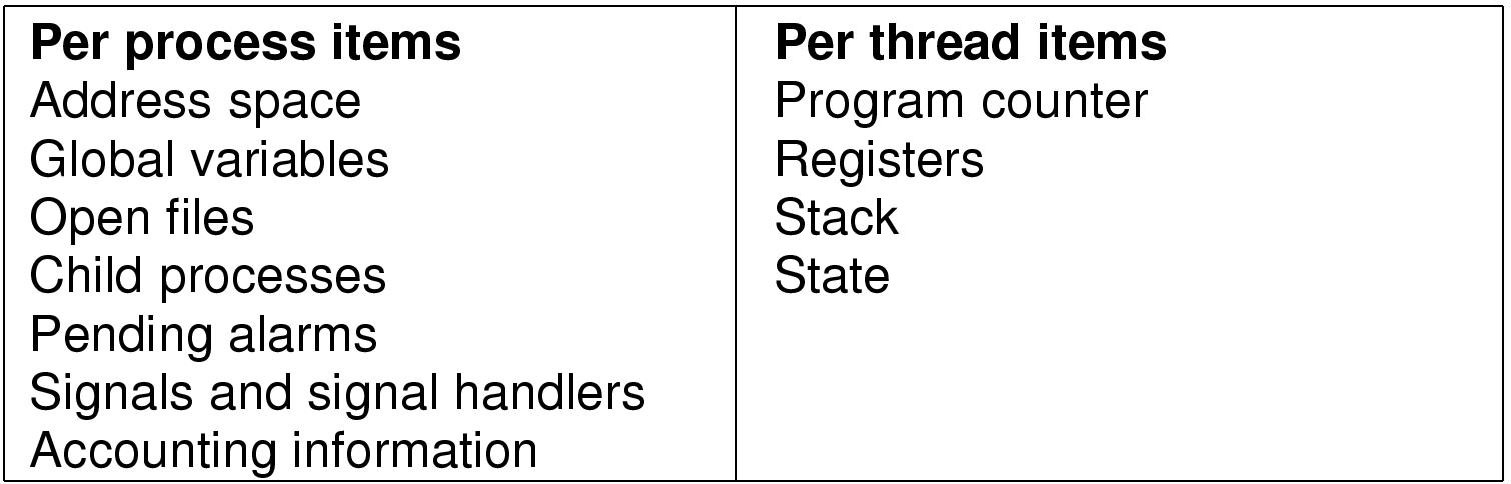
\includegraphics[scale=0.2]{mosv2f2-7}
  \end{center}
  \end{frame}

  \subsection{Single- and multi-threaded process}

  %% PAGE
  \begin{frame}
  \frametitle{Single- and multi-threaded process} \pause
  \begin{center}
    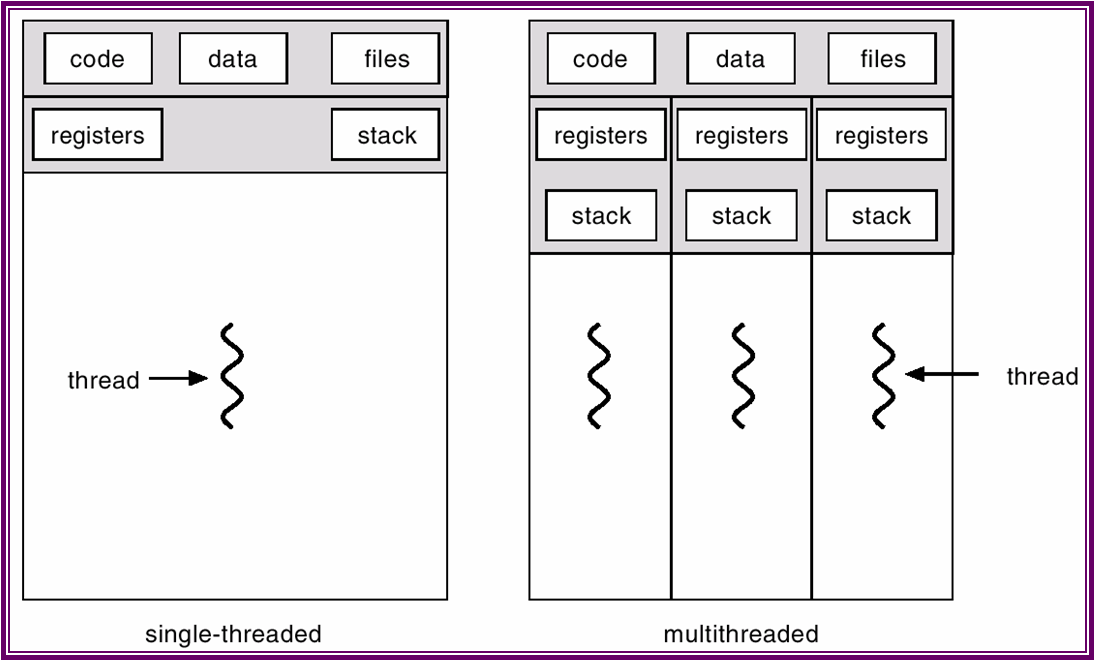
\includegraphics[scale=0.6]{v6f5-1}
  \end{center}
  \end{frame}

  \subsection{Benefits of thread}

  %% PAGE
  \begin{frame}
  \frametitle{Benefits of thread} \pause
  \begin{itemize}
  \item{Responsiveness} \pause
    \begin{itemize}
    \item{Allows other threads to continue responding to the user even if one or several threads is blocked or is performing a lengthy operation.} \pause
    \end{itemize}
  \item{Resource sharing} \pause
    \begin{itemize}
    \item{Since threads within the same process share memory and files, they can communicate with each other without invoking the kernel.} \pause
    \end{itemize}
  \item{Economy} \pause
    \begin{itemize}
    \item{Takes MUCH less time and resource to create a new thread than a process.} \pause
    \item{Takes MUCH less time to context switch threads within the same process.} \pause
    \end{itemize}
  \item{Utilization of multiprocessor architectures} \pause
    \begin{itemize}
    \item{Parallelism is possible by assigning each CPU a thread.}
    \end{itemize}
  \end{itemize}
  \end{frame}

  %% PAGE
  \begin{frame}
  \frametitle{Questions}
  \begin{itemize}
  \item{Any questions?}
  \end{itemize}
  \begin{center}
    
\includegraphics[scale=.5]{question}
  \end{center}
  \end{frame}

  \section{Thread implementation}

  %% PAGE
  \begin{frame}
  \frametitle{Thread implementation} \pause
  \begin{itemize}
  \item{Multi-threading can be implemented} \pause
    \begin{itemize}
    \item{at user space for \textbf{user threads};} \pause
    \item{at the kernel for \textbf{kernel threads}.} \pause
    \item{with a hybrid scheme by combining user- and kernel- threads.}
    \end{itemize}
  \end{itemize}
  \end{frame}

  \subsection{User thread}

  %% PAGE
  \begin{frame}
  \frametitle{User threads (1/2)} \pause
  \begin{itemize}
  \item{It's implemented outside of the kernel as a \textbf{thread library} at the user space.} \pause
    \begin{itemize}
    \item{It's the library which provides support for thread creation, scheduling and management.} \pause
    \item{As far as the kernel is concerned, it's managing ordinary, single-threaded process.} \pause
    \end{itemize}
  \item{Examples} \pause
    \begin{itemize}
%    \item{POSIX \textbf{Pthreads}} \pause
    \item{Mach \textbf{C-threads}} \pause
    \item{Solaris 2 \textbf{UI-threads}}
    \end{itemize}
  \end{itemize}
  \end{frame}

  %% PAGE
  \begin{frame}
  \frametitle{User threads (2/2)} \pause
  \begin{itemize}
  \item{Advantages of the user threads} \pause
    \begin{itemize}
    \item{Thread management and context switch need not to trap to the kernel.} \pause
      \begin{itemize}
      \item{This will save a lot of CPU cycles.} \pause
      \end{itemize}
    \item{Allow each process to have its own customized scheduling algorithm.} \pause
    \end{itemize}
  \item{Disadvantages of the user threads} \pause
    \begin{itemize}
    \item{Any user-level thread performing a blocking system call will cause the entire process to block.} \pause
      \begin{itemize}
      \item{Even if other threads are ready to run within the process.} \pause
      \end{itemize}
    \item{On a system with multiprocessors, the user-level threads cannot be dispatched for execution in parallel.}
    \end{itemize}
  \end{itemize}
  \end{frame}

  \subsection{Kernel thread}

  %% PAGE
  \begin{frame}
  \frametitle{Kernel threads} \pause
  \begin{itemize}
  \item{It's supported directly by the operating system.} \pause
    \begin{itemize}
    \item{The kernel performs thread creation, scheduling and management in kernel space.} \pause
    \end{itemize}
  \item{Examples} \pause
    \begin{itemize}
    \item{Windows NT/XP} \pause
    \item{Solaris} \pause
    %\item{Tru64 UNIX} \pause
    \end{itemize}
  \item{Advantages and disadvantages} \pause
    \begin{itemize}
    \item{Inverse of the user threads.}
    \end{itemize}
  \end{itemize}
  \end{frame}

  \iffalse

  \subsection{Multi-threading models}

  %% PAGE
  \begin{frame}
  \frametitle{Multi-threading models} \pause
  \begin{minipage}[c]{0.5\textwidth}
    \begin{itemize}
    \item{According to the implementation of the threads, there are three multi-threading models.} \pause
      \begin{itemize}
      \item{Many-to-One (Old Unix)} \pause
      \item{One-to-One (Windows)} \pause
      \item{Many-to-Many (Solaris)} \pause
      \end{itemize}
      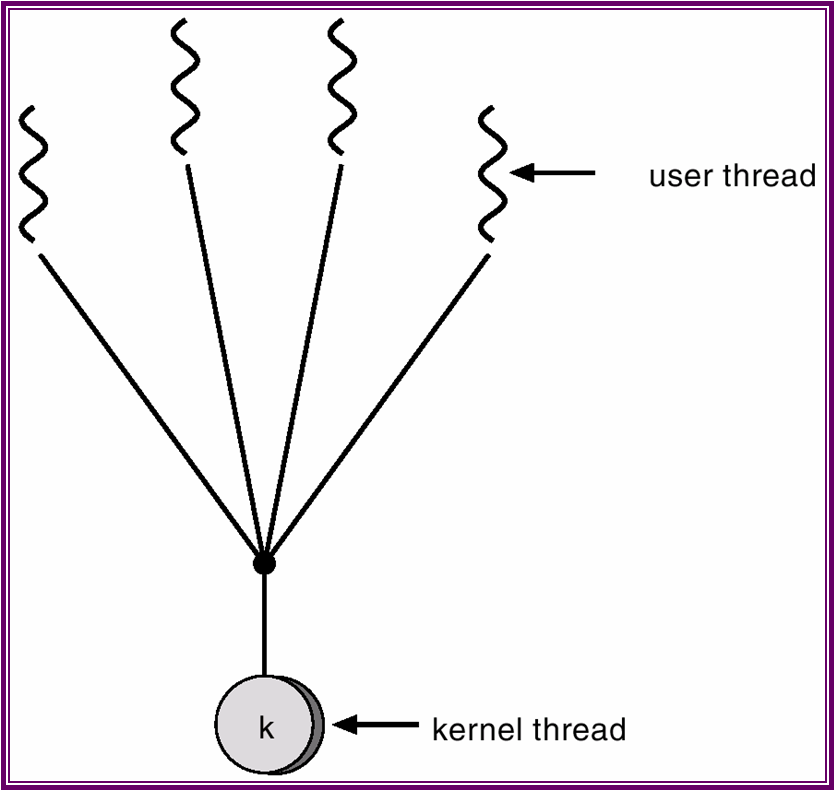
\includegraphics[scale=0.3]{v6f5-2} \pause
    \end{itemize}
  \end{minipage}%
  \begin{minipage}[c]{0.5\textwidth}
    \begin{center}
      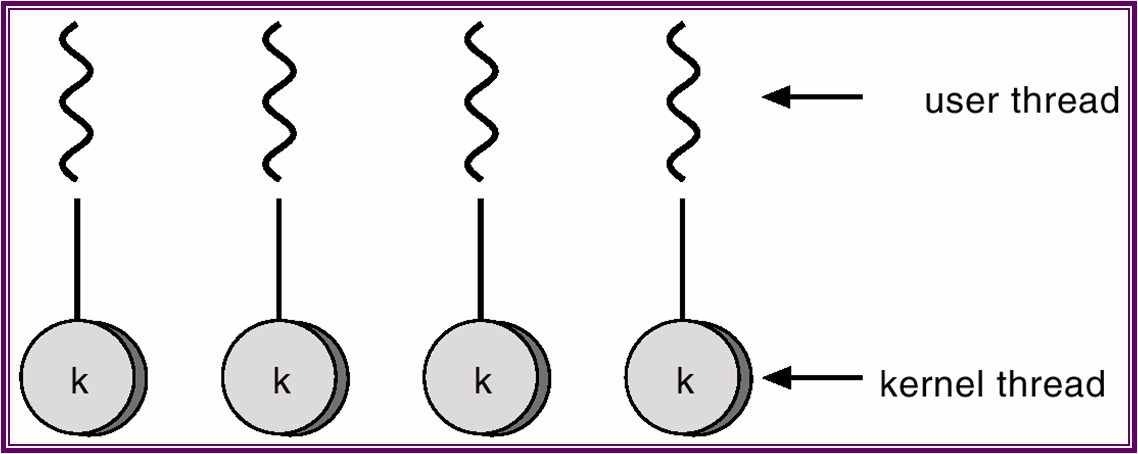
\includegraphics[scale=0.3]{v6f5-3}\\ \pause
      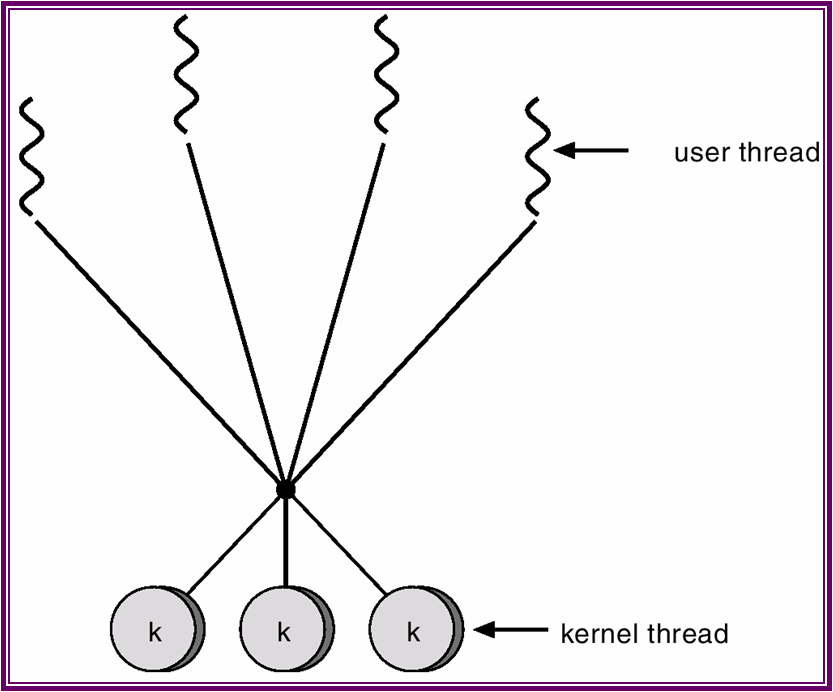
\includegraphics[scale=0.4]{v6f5-4}
    \end{center}
  \end{minipage}
  \end{frame}

  \fi

  %% PAGE
  \begin{frame}
  \frametitle{Questions}
  \begin{itemize}
  \item{Any questions?}
  \end{itemize}
  \begin{center}
    
\includegraphics[scale=.5]{question}
  \end{center}
  \end{frame}

  \section{Multi-threaded programming}

\iffalse

  %% PAGE
  \begin{frame}
  \frametitle{Multi-threaded programming} \pause
  \begin{itemize}
  \item{Application programming interfaces (APIs)} \pause
  \item{Writing multi-threaded code}
  \end{itemize}
  \end{frame}

\fi

  \subsection{Multi-threaded APIs}

  %% PAGE
  \begin{frame}
  \frametitle{Multi-threaded application programming interface} \pause
  \begin{itemize}
  \item{\textbf{Pthreads}} \pause
    \begin{itemize}
    \item{Pthreads refers to the POSIX\footnote{POSIX or ``Portable Operating System Interface for uniX'' is the collective name of a family of related standards specified by the IEEE to define the application programming interface (API) for software compatible with variants of the Unix operating system.} standard (IEEE 1003.1c) defining an API for thread creation and synchronization.} \pause
      \begin{itemize}
      \item{It's a \emph{specification} for thread behavior, NOT an \emph{implementation}.} \pause
      \end{itemize}
    \end{itemize}
  \item{Win32} \pause
    \begin{itemize}
    \item{CreateThread, ExitThread and TerminateThread, etc.} \pause
    \item{POSIX Threads for Win32 (http://sources.redhat.com/pthreads-win32)}
    \end{itemize}
  \end{itemize}
  \end{frame}

  \subsection{Pthreads}

  %% PAGE
  \begin{frame}[fragile]
  \frametitle{Example: Pthreads} \pause
  \begin{minipage}[c]{0.6\textwidth}

\begin{lstlisting}
#include <pthread.h>

int sum; /*shared variable*/

/*the thread function*/
void *runner(void *arg);

int main()
{
  pthread_t tid; /*thread ID*/
  pthread_attr_t attr; /*attributes*/

  /*get default attributes*/
  pthread_attr_init(&attr);

  /*create the thread*/
  pthread_create(&tid,&attr,runner,82);

  /*wait for the thread to exit*/
  pthread_join(tid,NULL);

  printf("sum = %d\n",sum);
}
\end{lstlisting}

  \end{minipage}%
  \begin{minipage}[c]{0.4\textwidth}
\lstset{frame=single}
\begin{lstlisting}
void *runner(void *arg)
{
  int i, upper=(int)arg;
  sum=0;
  if(upper>0)
     for(i=1;i<=upper;i++)
        sum+=i;

  pthread_exit(0);
  //or return (void *)0;
}
\end{lstlisting}

  \end{minipage}
\end{frame}

  \subsection{Win32 threads}

  %% PAGE
  \begin{frame}[fragile]
  \frametitle{Example: Win32} \pause
  \begin{minipage}[c]{0.6\textwidth}

\begin{lstlisting}
#include <windows.h>

int sum; /*shared variable*/

/*the thread function*/
DWORD WINAPI runner(LPVOID arg);

int main()
{
  DWORD tid; /*the thread ID*/
  HANDLE hThr; /*the thread handle*/

  /*create the thread*/
  hThr=CreateThread(0,0,runner,82,0,&tid);

  /*wait for the thread to exit*/
  WaitForSingleObject(hThr,INFINITE);

  printf("sum=%d\n",sum);
}
\end{lstlisting}

  \end{minipage}%
  \begin{minipage}[c]{0.4\textwidth}
\lstset{frame=single}
\begin{lstlisting}
DWORD WINAPI runner(LPVOID arg)
{
   int i, upper = (int)arg;
   sum = 0;
   if(upper > 0)
      for(i = 1; i <= upper; i++)
         sum += i;

  ExitThread(0);
  // or return 0L;
}
\end{lstlisting}

  \end{minipage}
\end{frame}

  %% PAGE
  \begin{frame}
  \frametitle{Questions}
  \begin{itemize}
  \item{Any questions?}
  \end{itemize}
  \begin{center}
    
\includegraphics[scale=.5]{question}
  \end{center}
  \end{frame}

\iffalse

  \subsection{Writing multi-threaded code}

  %% PAGE
  \begin{frame}
  \frametitle{Writing multi-threaded code} \pause
  \begin{itemize}
  \item{There are many tricks to write multi-threaded code. We will examine two of them:} \pause
    \begin{itemize}
    \item{Thread-specific data (Thread local storage, TLS)} \pause
    \item{Reentrant code}
    \end{itemize}
  \end{itemize}
  \end{frame}

  %% PAGE
  \begin{frame}
  \frametitle{Thread local storage (TLS) (1/2)} \pause
  \begin{itemize}
  \item{Threads belonging to a process share the data of the process.} \pause
    \begin{itemize}
    \item{This is one of benefits of multi-threaded programming.} \pause
    \end{itemize}
  \item{However, each thread might need its own copy of certain data in some circumstances.} \pause
    \begin{itemize}
      \begin{minipage}[c]{0.4\textwidth}
      \item{For example, in the Unix/Linux, when a process makes a system call that fails, the error code is put into a global variable \emph{errno}. It can be inspected later to determine the reason of failure.} \pause
      \end{minipage}%
      \begin{minipage}[c]{0.6\textwidth}
        \begin{center}
          \includegraphics[scale=0.4]{errno}
        \end{center}
      \end{minipage}
    \end{itemize}
  \end{itemize}
  \end{frame}

  %% PAGE
  \begin{frame}
  \frametitle{Thread local storage (TLS) (2/2)} \pause
  \begin{itemize}
  \item{Various solutions to this problem are possible.} \pause
    \begin{itemize}
    \item{Prohibit global variables altogether.} \pause
    \item{Assign each thread its own private global variables, i.e., \textbf{thread local storage}.} \pause
    \end{itemize}
  \item{Examples} \pause
    \begin{itemize}
    \item{Pthreads library provides API support for TLS.} \pause
    \item{Win32 also includes \emph{TlsAlloc/TlsFree/TlsGetValue/TlsSetValue} to allocate and access the TLS.} \pause
    \item{Latest C/C++ compilers (such as MSVC and GCC) add a new storage class \emph{\_\_thread} to declare global/static variables as TLS directly.} %FIXME
    \end{itemize}
  \end{itemize}
  \end{frame}

  %% PAGE
  \begin{frame}
  \frametitle{Reentrant code}
  \begin{itemize}
  \item{A piece of code is NOT reentrant,} \pause
    \begin{itemize}
    \item{if it's NOT designed to have a second call made to it while a previous call has NOT yet finished.} \pause
    \item{For example, a function manipulating (inserting or deleting) a global singly-linked list.} \pause
    \end{itemize}
  \item{Solution: synchronization} \pause
    \begin{itemize}
    \item{Will be covered in chapter 7.}
    \end{itemize}
  \end{itemize}
  \end{frame}

  %% PAGE
  \begin{frame}
  \frametitle{Questions}
  \begin{itemize}
  \item{Any questions?}
  \end{itemize}
  \begin{center}
    
\includegraphics[scale=.5]{question}
  \end{center}
  \end{frame}

\fi

  %% PAGE
\end{CJK*}
\end{document}
